\chapter{Design}
\label{sec:design}

% Ist das zentrale Kapitel der Arbeit. Hier werden das Ziel sowie die
% eigenen Ideen, Wertungen, Entwurfsentscheidungen vorgebracht. Es kann
% sich lohnen, verschiedene Möglichkeiten durchzuspielen und dann
% explizit zu begründen, warum man sich für eine bestimmte entschieden
% hat. Dieses Kapitel sollte - zumindest in Stichworten - schon bei den
% ersten Festlegungen eines Entwurfs skizziert werden.
% Es wird sich aber in einer normal verlaufenden
% Arbeit dauernd etwas daran ändern. Das Kapitel darf nicht zu
% detailliert werden, sonst langweilt sich der Leser. Es ist sehr
% wichtig, das richtige Abstraktionsniveau zu finden. Beim Verfassen
% sollte man auf die Wiederverwendbarkeit des Textes achten.

% Plant man eine Veröffentlichung aus der Arbeit zu machen, können von
% diesem Kapitel Teile genommen werden. Das Kapitel wird in der Regel
% wohl mindestens 8 Seiten haben, mehr als 20 können ein Hinweis darauf
% sein, daß das Abstraktionsniveau verfehlt wurde.

% Die Lösung kurz vorstellen. also du hast dich für die lösung mit dem dc network entschieden und das wurde bisher noch nicht vorgeschlagen in der wissenschaft. Dann sagen bevor du das prinzip vorstellt werden erstmal alle Teilnehmer, die in dem System vorkommen, vorgestellt. dazu auch das bild aus der technischen richtlinie benutzen, wo smartmeter und smart meter admin. welche netzwerke also han etc...
%Dann sagen, dass du erstmal auf das angreifermodell eingehst und dann dc netz erklären und dann die lösung vorschlagen.
%die lösung wurde noch nicht diskutiert, weil in der wissenschaft immer davon ausgegangen wurde, dass smart meter nicht sicher sind,wir gehen davon aus, dass ein smart meter vertraut werden kann und das man deshalb auch nicht auf das billing eingehen muss, weil das smart meter korrekt arbeitet und das billing deshalb trivial ist. der stromanbieter kann auch prüfen  bzw. die logeinträge sind fälschungssicher.

This chapter outlines the conceptual solution of this thesis to achieve privacy-preserving smart meters. The proposed protocol can be categorized as aggregation without a trusted third party. Before discussing the conceptual solution, the technical guideline from the BSI will be explained. The BSI is the cyber-security authority of the German government and is responsible for critical infrastructures such as smart grids in Germany.  The technical guideline TR-03109 resolves all security standards and security concepts that must be met by all power grid providers in Germany. Therefore, the technical guideline gives a good overview of the actual structure of the German power grid. After getting an overview of the power grid and its participants, an attacker model will be designed. The attacker model will introduce all necessary participants, what their motives are and what malicious motives they might pursue. Finally, the security protocol will be presented. It will be shown how the protocol can be integrated into the technical policy and how different potentially malicious participants are handled.

\section{Technical guideline TR-03109}
This paragraph will discuss the technical guideline published by the BSI (Federal Office for Information Security). The BSI is the entity of the German federal government that deals with digital security issues and issues recommendations as well as mandatory security guidelines for critical infrastructures. Among other things, technical guidelines are published in which security standards are defined for different IT systems. The technical guideline BSI-TR-03109 defines minimum requirements for the functionality, security and interoperability of smart meters in Germany.  The technical guideline BSI-TR-03109 defines minimum requirements for functionality, security and interoperability that individual components of smart meters in Germany must fulfill. The guideline as a whole consists of 6 different documents, which are shown in Figure 3.1. Based on the guidelines, it is possible to have devices certified by test centers. Unless otherwise described, all information are derived from the technical guideline.\\
\\
\textbf{Actors on the SMGW}
\\
\\
Consumer: The consumer is the person who uses electrical energy, gas, water
or heat. In addition, the consumer is the owner of the measurements processed and stored in the SMGW. In order to interact with the SMGW, the consumer uses a communication device. All necessary data can be retrieved and displayed through it.\\
SMGW administrator:
A Smart Meter Gateway Administrator (GWA) a trusted entity and each SMGW is assigned a GWA. The GWA handles the configuration, monitoring and control of SMGWs and it is even possible to perform updates of SMGWs via the GWA.\\
Authorized external entities:\\
External market participants (EMT) are all other authorized participants in the energy network that can establish a communication connection with the SMGW.These include power grid providers and electricity suppliers. The SMGW ignores all other communication requests that do not come from the GWA or EMTs in order to prevent attacks.\\
There are several other actors such as Controllable Local Systems, service technicians and meters. However, these actors do not play a major role in the protocol that is proposed here.
\begin{figure}[tbp]
  \centering
  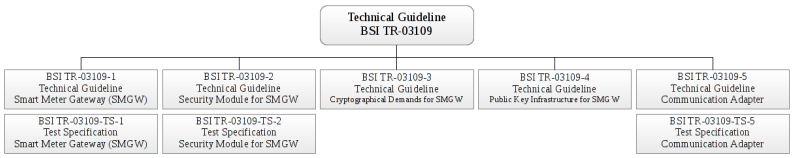
\includegraphics[width=1\textwidth]{images/BSI-TR-03109.png}
  \caption[Short description]{An example of a NILM analysis.}
  \label{fig:Appliance_Model}
\end{figure}
\\
\\
\textbf{Interfaces and functions of the Smart Meter Gateway}
\\
\\
A smart meter or as described in the technical guideline a smart meter gateway(SMGW) must provide 3 different physical interfaces.
\begin{enumerate}
\item Local Metrological Network (LMN):\\
The LMN is the communication interface in which communication takes place with the connected meters for energy and material quantities (electricity, gas). An SMGW can communicate with one meter from one end user or with several meters from different end users. In practice, however, one SMGW is often responsible for one meter. The measured values are sent from the meters via the LMN to the SMGW and stored there.
\item Wide Area Network (WAN):\\
The WAN is the only communication interface with which the SMGW can communicate with EMTs or GWAs over the Internet. If a request is made to the SMGW that was not sent by these authorized participants, then the request is discarded and ignored.
\item Home Area Network (HAN):\\
In HAN, an SMGW interacts with Controllable Local Systems (e.g., photovoltaic systems). In addition, users and service technicians can use the HAN interface to display information about power consumption through functions offered by the SMGW.
\end{enumerate}
\textbf{Functionality of the smart meter gateway}
\\
\\
First, the task of SMGW is to store the measurements sent by meters from the LMN. Then, the readings are processed in the SMGW and sent to the authorized EMTs in the WAN after processing. An SMGW must also perform the tasks of a firewall and separate the 3 interfaces. It is therefore impossible for an EMT or GWA to make requests to devices located in the HAN or LMN, even if it is allowed to interact with the SMGW over the WAN.
Since the WAN interface is the most important interface for this work, it will be discussed in more detail.\\
\\
\textbf{Functions of the SMGW in the WAN}
\\
\\
The tasks performed by the WAN have already been explained in the paragraph above. Now the functions and security mechanisms offered by the SMGW to guarantee secure interaction on the WAN will be described.
\begin{enumerate}
\item Transmission of measured values based on evaluation and WAN communication profiles:\\
Communication profiles of GWAs are stored in SMGW. The communication profiles determine how the data is processed in the SMGW and forwarded to EMTs.

\item Pseudonymization:\\
Data that is not relevant for billing must be pseudonomized for data protection reasons. For this purpose, the unique identification number that each SMGW has is replaced by a pseudonym. Subsequently, the information is not sent directly to an EMT, but is forwarded to the EMT via the GWA. This additionally protects the identity of the sending SMGW.%vllt als extra part machen. was unten kommt.
Even if peusodonymization does not allow an SMGW to be directly assigned, the described attack in [ref] and the resulting behavioral analysis is still possible. Since no other security mechanisms are available from the SMGW, the question must be asked whether pseudonymization as proposed in the technical guideline is sufficient.

\item Time synchronization:\\
In order for the cost electricity consumption to be calculated correctly, it is essential that the SMGW have an accurate time. For this purpose, the system time of the SMGW is synchronized with the time server of the GWA at regular intervals.

\item Wake-Up Service:\\
A GWA is able to force a communication link with the SMGW. This is done via a data packet signed by the GWA. The SMGW then establishes a fixed preconfigured communication connection to the GWA. This enables the GWA to execute administration commands on the SGMW. 
\end{enumerate}
\section{Adversary Model}
It has already been explained in this chapter which participants in the power grid interact with each other. Now in particular it will be discussed which motives the different participants have and which malicious motives can be pursued by the participants or by attackers.  \\
\\
The smart meter attempts to achieve the 3 security objectives of confidentiality, integrity and availability. The 3 security goals are often summarized as CIA.
\subsection{Customer Motives}
The most important goal for the customer is the guarantee of anonymity through the smart meter. Possible attacks on the electricity consumption penetrate deeply into the private sphere of each customer. Therefore, no conclusions may be drawn from the electricity consumption of a customer.

\todo{write design}

\cleardoublepage

%%% Local Variables:
%%% TeX-master: "diplom"
%%% End:
